
\chapter{Detail Preserving Continuum Simulation of Straight Hair}
%
%Simulating hair on a virtual character remains one of the most
%challenging aspects of computer graphics. As hair is an integral
%part of creating many virtual characters, the problem is especially important.
%Unfortunately, the massive number of hairs interacting and colliding
%makes this task especially challenging. Many approximations for
%simulating hair exist, but they typically fail to provide the amount of
%detail that real hair exhibits. Several applications, such as feature
%films, aim to capture the high degree of complexity caused by several 
%thousand interacting hair strands.


Even though individual hair dynamics scale well to multiple hairs (as each hair
is dynamically decoupled), accurately simulating many hairs interacting with
each other remains a challenge.  Instead, numerous approaches have been
developed to manage the complexity of many hairs interacting by simulating a
smaller set of guide hairs (typically no more than several hundred) that
interact with large repulsion forces, interpolating a larger number of hairs for
rendering. This leads to very efficient simulation times, but a limited amount
of hair detail is captured (ignoring stray hairs such as the
so-called ``flyaways'') because, essentially, each guide hair represents
hundreds (or even thousands) of actual hairs.

Alternatively, there have been several methods that treat every simulated hair
as part of a fluid-like continuum volume. These approaches naturally model hair
interaction without explicit collisions. However, the downside is that intricate
features of individual hairs are lost because each hair is enslaved to the
continuum.


\begin{figure}[!ht]
  \centering
  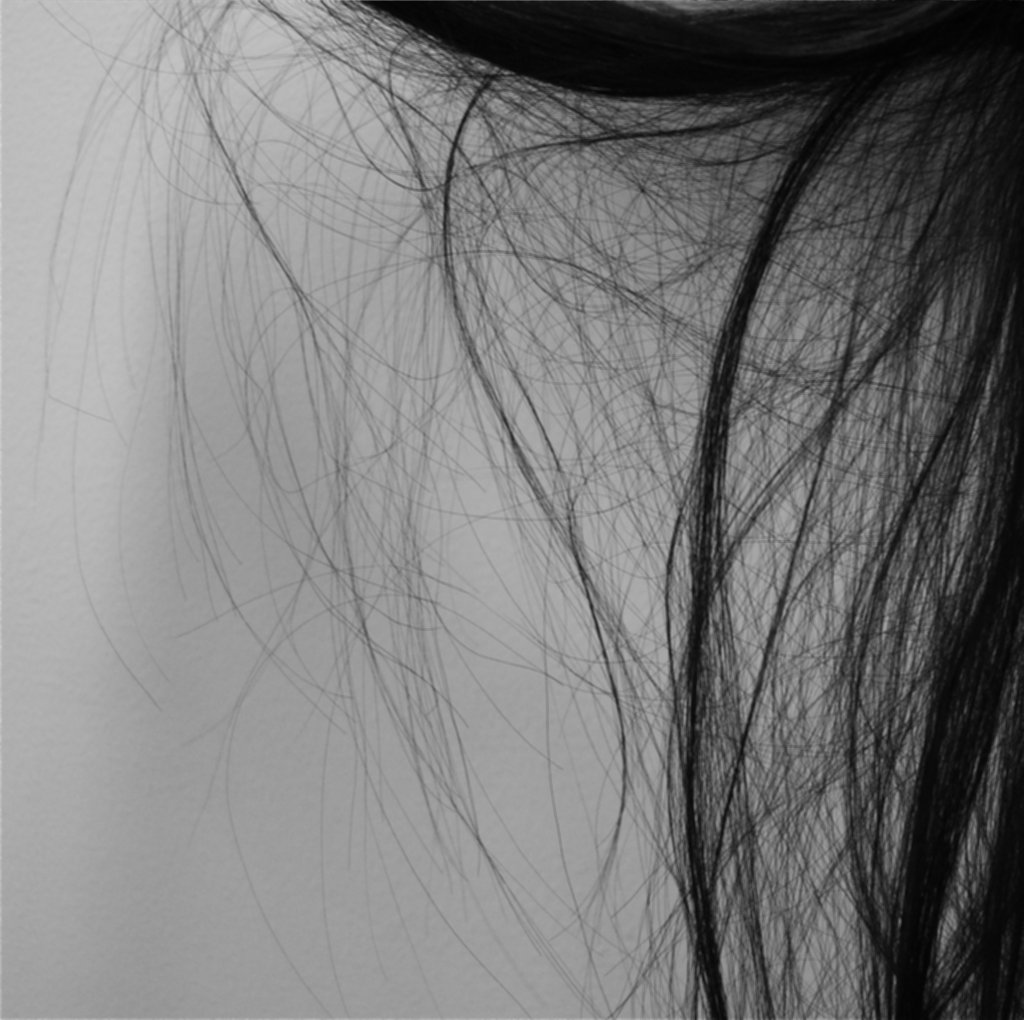
\includegraphics[height=.48\linewidth]{hair/images/realhair_1024}
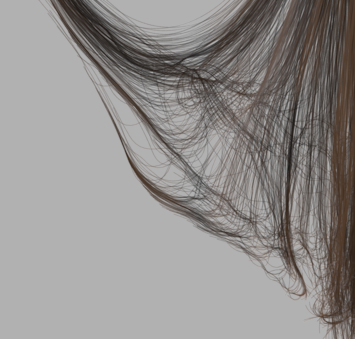
\includegraphics[height=.48\linewidth]{hair/images/tubes-alone-cropped-116}
  \caption{\label{fig:hold} (Left) Real hair exhibiting an intricate webbed
appearance resulting from complex collision and contact. (Right) Our method
creating a similar effect by using a
    combination of Eulerian and Lagrangian collision techniques.}
\end{figure}

Our technique factors hair computation into two parts: a coarse, highly coupled
volumetric behavior, which is efficiently modeled by a continuum; and
a finer, more locally coupled Lagrangian particle simulation of
hair. Unlike previous continuum-based approaches that only simulate
guide hairs that do not interact directly, our method simulates many
hairs (several thousand) that are allowed to collide directly (as well
as through the volume). We handle self-collisions more efficiently
than fully Lagrangian collision models because the volume does most of
the work towards resolving collisions.  Thus, our method can capture the
intricate details of many individual strands while efficiently
maintaining the overall hair volume. 
%

%\vspace{-2pt}
%\section{Related Work}
%\vspace{-4pt}
%
%Hair modeling is an active area of research that can be divided into
%the following categories: hair shape modeling, hair strand dynamics,
%hair complexity management and interaction, hair shading and self-shadowing.
%Static hair shape
%modeling, such as
%\cite{yu:2001:model-hairstyle,kim:2002:hair,choe:2005:statistical-wisp}, hair
%shading and shadow
%computation are beyond the scope of our paper, so we do not discuss them
%further. A
%more detailed discussion on these topics can be found in the recent
%survey paper \cite{ward:2007:hairsurvey}.

%\textbf{Strand Dynamics.} Many hair simulation techniques consider different geometric and constitutive models
%for modeling individual hair strands or clumps of hair starting with
%mass spring systems \cite{rosenblum:1991:hair} and projective dynamics
%\cite{anjyo:1992:hair}.  Mass/spring simulated lattice deformers can
%be added to model torsion
%\cite{plante:2002:hair-complexity,selle:2008:hair}.
%Rigid body chaining methods are also commonly used
%\cite{brown:2004:real-time-knot,choe:2005:simulating-complex-hair,hadap:2006:orientedstrands}.
%Techniques based on elastic rod theory have become popular
%starting with \cite{pai:2002:strands} and continuing with
%\cite{gregoire:2006:interactive-simulation-one-dimensional,bertails:2006:superhelices}.
%\cite{spillmann:2007:corde} also uses elastic rod theory but
%adaptively changes the number of points that define the hair curve.
%Most recently, \cite{bergou:2008:elastic-rods} provides a novel
%modeling of twist as deviation from a canonical frame as well as a
%method to evolve this separately quasistatically. Work in strand
%dynamics has been extensive, and our technique can be used with the
%practitioner's model of choice, but for simplicity we use
%the mass/spring model.
%
%\textbf{Hair Interaction and Complexity.}
%The simplest (but most expensive) approach to hair complexity
%management is simulating and rendering every hair
%\cite{rosenblum:1991:hair,anjyo:1992:hair,selle:2008:hair}. While this
%theoretically yields the most detail, it is the most intractable,
%especially if self-collisions are considered.  Thus most practitioners
%use a clumping or continuum level of detail scheme that trades
%accuracy for computational tractability:


\begin{figure}[t!]
  \centering \fbox{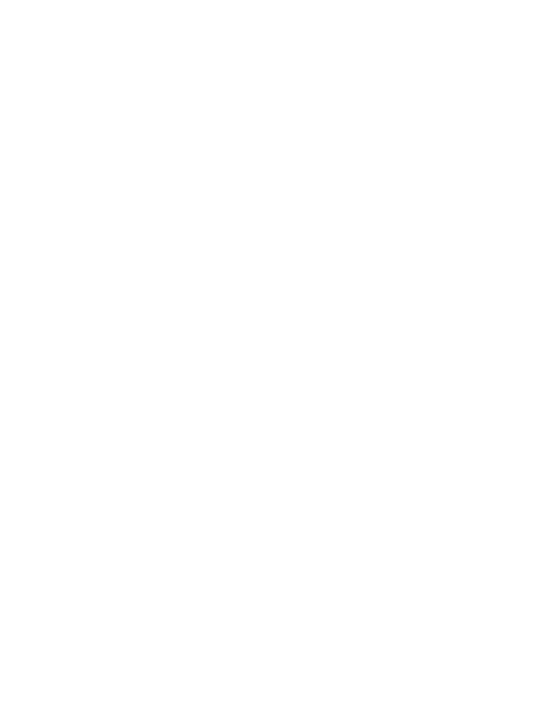
\includegraphics[height=.4\linewidth]{hair/images/viz/curves-15}} \fbox{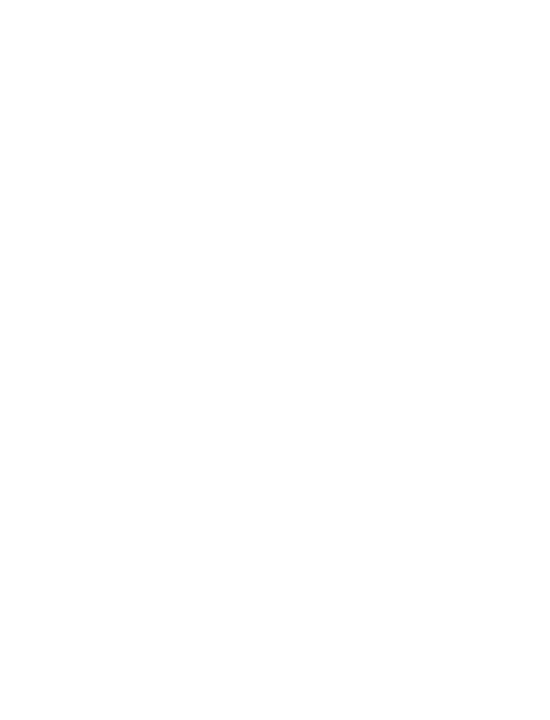
\includegraphics[height=.4\linewidth]{hair/images/viz/velocities-15}}
  \caption{\label{fig:viz} Our method models the hair both as curves
    (left) and as a volumetric velocity field (right).}
\end{figure}
%
%\textbf{Continuum models.}  \cite{hadap:2001:continuum-hair} uses a Lagrangian
%fluid (smoothed particle hydrodynamics) technique to model fluid forces on a
%mass/spring system. While this efficiently handles bulk behavior, detailed hair
%behavior is lost. In addition, since smoothed particle hydrodynamics (SPH) is
%used, forcing fluid interaction through spring like forces, this approach is
%effectively as numerically difficult as standard self-repulsion spring forces.
%\cite{bando:2003:hair-loosely-connected-particles} also uses a continuum
%approach while discarding particle connectivity for real-time
%applications. Unfortunately, this results in visual artifacts in renderings
%because of the lack of connectivity in addition to the continuum's loss of high
%fidelity detail.  \cite{petrovic:2005:levelset-hair} presented a continuum
%approach that rasterized hair to an Eulerian velocity field and level set with
%the goal of reducing computational complexity, rather than improving on
%fidelity. Dynamics on the grid was limited to repeated averaging (an
%approximation of viscosity) to obtain friction effects. Unlike our method,
%they did not consider the incompressibility or other fluid behaviors that could
%be imparted on the velocity field. In addition, the goal of the work was to
%model relatively simple hairstyles on stylized characters, so the detail lost by
%using a coarse grid was acceptable for their application.

%\textbf{Clumped models.}  There are many techniques that simulate hair
%interactions through a sparse set of disjoint guides that collide with one
%another
%\cite{bertails:2006:superhelices,hadap:2006:orientedstrands,gupta:2006:real-time-hair,chang:2002:mutualinteractions}.
%A greater set of rendered hair strands are then either interpolated between
%these guides or clumped to the guide strands.
%\cite{plante:2002:hair-complexity} used a lattice whose vertices were simulated
%with a mass/spring model to define many more interpolated
%hairs. \cite{choe:2005:simulating-complex-hair} synthesized additional hairs
%from a sparse set of simulated guide hairs with a statistical
%model. \cite{bertails:2006:superhelices} used a combination of interpolation and
%clumping to generate rendered strands.  Many clumped techniques also use
%adaptivity to merge or split groups of hair to reduce computation where and when
%the required detail is low
%\cite{bertails:2003:adaptive-wisp-tree,ward:2003:modeling-hair-lod,ward:2003:adaptive-grouping-hair}. The
%use of sparse clumps often allows the use of cheap repulsion penalties as
%opposed to geometric collisions because guides are expected to have
%thickness, and in Section~\ref{sec:collisions} we will discuss how this breaks
%down with thousands of guides.



\vspace{-2pt}
\section{Method Overview}
\vspace{-4pt}

Our approach combines a Lagrangian hair solver with an Eulerian fluid simulator
(see Figure~\ref{fig:viz}).
We use a mass/spring model for the hair particles, connecting each particle in
sequence with a spring and every other particle with a bending spring.  Torsion
could be added to the mass/spring model, or a different strand model (such as an
articulated rigid body or Cosserat model) could be used. Each time integration step of the
dynamic system proceeds as follows (see Figure~\ref{fig:outline}):


{
\begin{enumerate}
\item Save collision-free position and velocity
\item Velocity step ${v}^{\star n+1}_i = {v}_i^n + \Delta t a_i(x^n_i,{v}^{\star  n+1}_i)$
\item Use the volume technique to modify $v^{\star n+1}_i$ into a corrected velocity
  $\hat{v}^{n+1}_i$  (Substeps 3a, 3b, 3c)
\item Modify $\hat{v}^{n+1}_i$ for collisions to get $v^{n+1}_i$ 
\item Compute final position $x^{n+1}_i = x^n_i + \Delta t v^{n+1}_i$
\end{enumerate}
}
where $x^n_i$, $v^n_i$ is the time $t_n$ position and velocity of the $i$th
particle, respectively, and $\Delta t$ is the time step. Note that step 4
is discussed in Section~\ref{sec:collisions} and implemented using
\cite{bridson:2002:cloth}.  $a_i(x^n_i,v^{\star n+1}_i)$ is separated into a linear
damping part and non-linear elastic part as in \cite{bridson:2003:cloth} to
preserve elastic modes. Step 3 rasterizes the hair volume to a grid representing
the hair density and velocity, modifies the velocity field to handle bulk
self-interaction and then applies the modified information back to the particle
velocities (Section~\ref{sec:volume}).




\begin{figure}[t!]
  \centering
  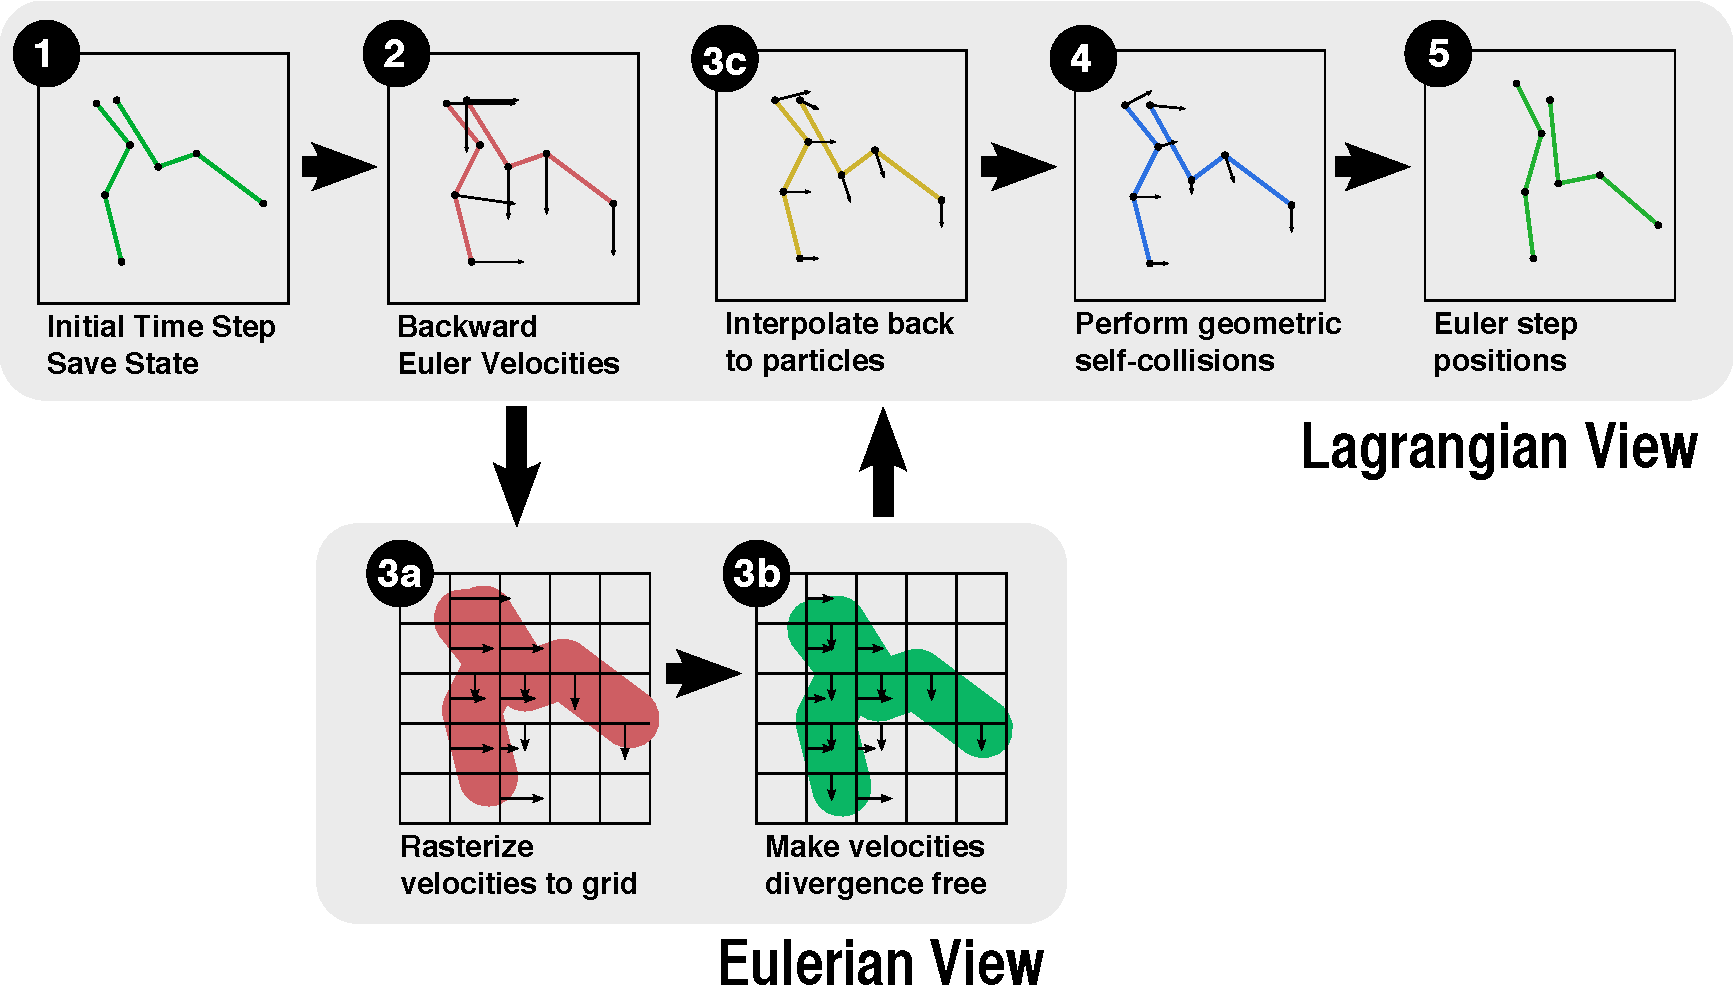
\includegraphics[width=1\linewidth]{hair/figures/redraw_geometric}
  \caption{\label{fig:outline} Outline of the Lagrangian (top) and Eulerian
    (bottom) components of our method.} 
\end{figure}

\vspace{-2pt}
\section{Solver}

\vspace{-5pt}
\subsection{Volume}
\vspace{-5pt}
\label{sec:volume}

A volume method is an ideal way to handle self-interaction of many hairs because
when many hairs are near each other, their contact and collisions allow a
propagation of any force through hairs in contact.  This behavior is similar to
the behavior of a fluid, which conserves momentum and mass. For
computational efficiency, we draw on incompressible fluid simulation
techniques to model our hair volume.  Density modeling is still
possible as discussed later in Section~\ref{sec:density}.

%For computational
%efficiency, we model the hair as an incompressible fluid in contrast to the
%compressible flow \cite{hadap:2001:continuum-hair} (standard SPH effectively
%only handles compressible flow see \cite{premoze:2003:particlefluids}). Density
%modeling is still possible as discussed later in Section~\ref{sec:density}.

The two common approaches used to model fluid volumes are Lagrangian
techniques (smoothed particle hydrodynamics, vortex particle methods)
and Eulerian techniques (common pressure/velocity incompressible
solvers such as \cite{Stam:1999:SF}). Eulerian techniques tend to be more efficient because nearest neighbor
searches are unnecessary.  The downside of Eulerian approaches is that
they are most natural on uniform grids that limit the amount of detail
available. Even particle based methods actually limit detail, because high
degree unstructured stencils also create numerical smoothing. For our purposes,
we will use an Eulerian approach and compensate for this lack of
detail by using high resolution Lagrangian collision handling techniques to
capture high fidelity detail.

An increasingly popular approach for fluid advection is the FLIP method
(introduced to graphics by \cite{zhu:2005:sand}) which replaces the traditional
Eulerian advection equation of velocity $v_t+v \nabla\cdot v=0$ with a
Lagrangian step $x_i^{n+1}=x_i^n+\Delta t v^n_i$. This velocity is
rasterized to a grid and made divergence free using the Chorin
projection method \cite{chorin:1967:ANM}. The divergence free velocity field is compared to the
original grid velocity field, and this difference is interpolated to the
particles and applied as an impulse.  This can be thought of as a
particle fluid method
that uses incompressible techniques to provide an implicit modeling of
incompressible behavior rather than an explicit one,
 %(which is analogous to \cite{baraff:1998:largesteps}'s use of
 %backward Euler instead of forward Euler for cloth). 
providing a convenient way to
communicate between the grid and particles. In fact, \cite{losasso:2007:sph}
demonstrate a hybrid grid/particle fluid technique that uses FLIP as a coupling
mechanism between the grid and the particles. Given the input candidate velocities $v^{\star n+1}_i$ and positions
$x^n_i$ from step 2, we follow steps similar to \cite{losasso:2007:sph},
though it is important to note our candidate positions contain the effects of
elasticity. 

At each timestep, we resize our grid to fit the volume of hair,
keeping the grid spacing constant.  We then rasterize candidate time
$t^{n+1}$ \emph{segments} at their candidate locations defined
by forward Euler, instead of \emph{particles} directly, to ensure good coverage of the
volume.  Consider a segment with particles $(i,j)\in S$ at its candidate
positions (i.e. $(x'_i,x'_j)=(x^n_i+\Delta t v^{\star n+1}_i$,$x^n_j+\Delta t
v_j^{\star n+1})$). Given a point $x$ in space which has distance $d_{ij}(x)$ to the
segment, define a weight 
$w_{ij}(x)=\max\left(0,r-d_{ij}(x)\right),$
where $r$ is a user-defined radius of influence for each segment.  We typically
used $r=3\Delta x/2$ in our simulations where $\Delta x$ is the grid
size. Then the rasterized velocity at any point is
$$v(x)= \frac{\sum_{(i,j)\in S} w_{ij}(x)[ (1-\alpha_{ij}(x)) v_i +
    \alpha_{ij}(x) v_j ]}{\sum_{(i,j)\in S} w_{ij}(x)}$$
where $\alpha_{ij}(x)$ is the interpolation fraction of the closest point on the
segment. Velocities and weights are computed on the faces (for MAC velocities)
and cell centers for density control and separation condition computation. 


\begin{figure}[t]
  \centering
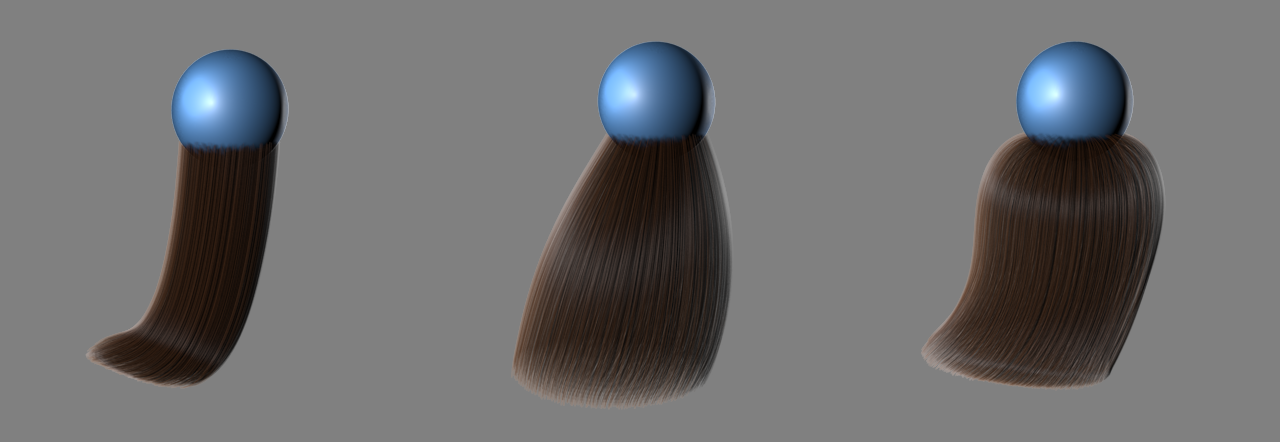
\includegraphics[width=.99\linewidth]{hair/images/density/density-figure}
  \caption{\label{fig:density} A demonstration of volumetric density
    control. (Left) high density and low volume. (Middle) moderate density and
    moderate volume. (Right) low density and high volume.}
\end{figure}

Once the velocities and weights are rasterized, we must setup a
Poisson system $\nabla^2p=\nabla \cdot v_\textrm{grid}^{\star n+1}$ to
project the grid velocities to be divergence free in step 3b. Any cell
with a weight lower than a threshold is set as a Dirichlet $p=0$
condition, and any face that is inside a kinematic collision body is
given a zero Neumann boundary condition and the velocity on that face is set to
the object velocity. A divergence source term is set to target density
(see Section~\ref{sec:density}). We solve the system with
preconditioned conjugate gradient and then compute the divergence free
velocity field $v^{n+1}_\textrm{grid}=v_\textrm{grid}^{\star
  n+1}-\nabla p$. Additional viscosity could also be added at this stage to
create additional friction (variable viscosity is also a
possibility, see \cite{Carlson:2002:MAF,rasmussen:2004:t3}).

Finally, in step 3c, FLIP is used to apply this velocity back to the $i$th
particle using the formula
$$\hat{v}_i^{n+1} =\xi \left[v_i^{\star n+1} +
(I(x_i^n,v_\textrm{grid}^{n+1}-v^{\star n+1}_\textrm{grid}))\right] +(1-
\xi)  I(x_i^n,v_\textrm{grid}^{n+1})$$ where $I(x,v)$ is trilinear
interpolation at location $x$ of a vector field $v$ and $\xi$
controls the amount of FLIP vs. PIC.  In our simulations, we typically
used a value of $\xi=.95$.

\vspace{-5pt}
\subsubsection{Density Control}
\label{sec:density}
\vspace{-5pt}

The rasterized cell weights are used to define a density which can be targeted
to a user defined density as in \cite{losasso:2007:sph} by using a divergence
source term in the Poisson equation. Near collision objects this method can lose
effectiveness because kinematic velocity constraints interfere with
divergence. Thus, we also modify the fixed velocities on Neumann faces if the
face's weight is less than the density target.  We simply add to the constrained
velocity in the collision body's normal direction. This is analogous to a
penalty repulsion in Lagrangian dynamics, but handling it in the Poisson
equation means it will be made consistent globally.  The results of density
control can be seen in Figure~\ref{fig:density}.

\vspace{-5pt}
\subsubsection{Separation Control}
\vspace{-5pt}

\begin{figure}[t]
  \centering
\includegraphics[width=.99\linewidth]{hair/images/separation/separation-figure}
  \caption{\label{fig:separation} A volumetric separation constraint can be
    defined to control the amount of sticking. (Left) no separation condition is
  applied. (Right) an easy to satisfy separation condition is specified to
  produce immediate decoupling.}
\end{figure}


\begin{figure*}[htb]
  \centering
  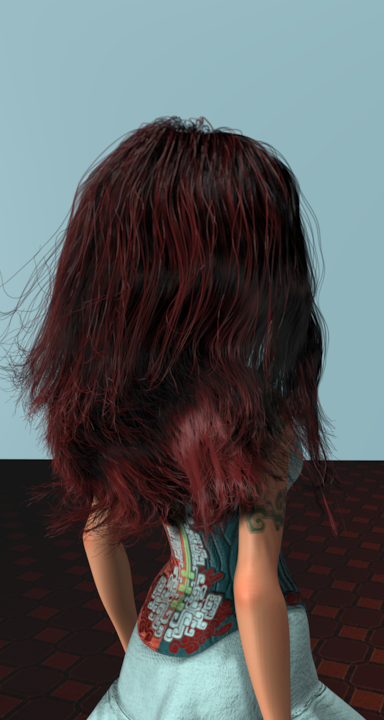
\includegraphics[height=.288\linewidth]{hair/images/character/hair-5}
  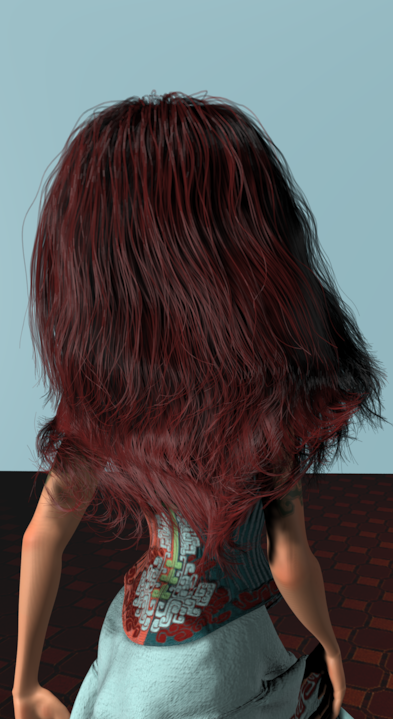
\includegraphics[height=.288\linewidth]{hair/images/character/hair-10}
  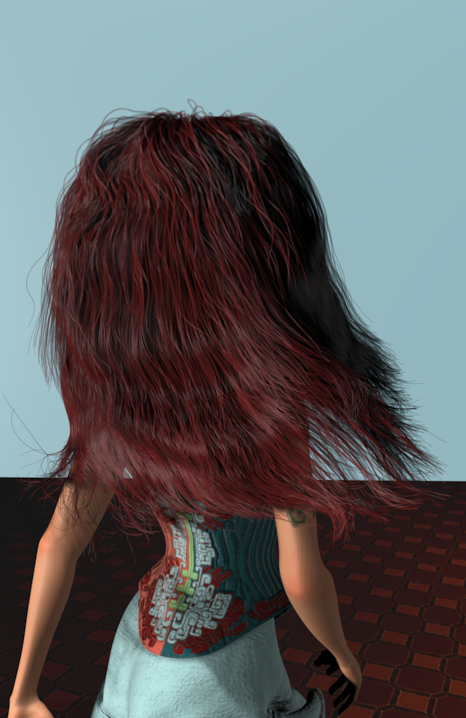
\includegraphics[height=.288\linewidth]{hair/images/character/hair-12}
  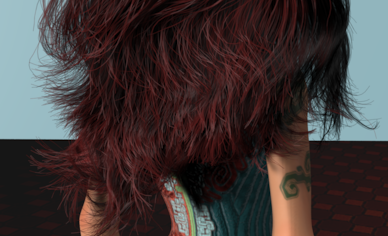
\includegraphics[height=.288\linewidth]{hair/images/character/hair-close-7}
  \caption{\label{fig:char} A hand-animated character walking with a hairstyle
    simulated by our method. The rightmost image is a closeup. Images \copyright
  Disney. All Rights Reserved.}
\end{figure*}


A problem with volume/continuum approaches to hair is that nearby hairs are
forced to behave similarly. This is desired when hair is under compression
because it forces the velocity to be zero at the center, preventing
interpenetration. However, when two regions of hair have disparate
velocity fields, it may be desirable to control the amount of sticking
this artificial coupling can create (Figure~\ref{fig:separation}). In
fact, this problem also appears in fluid techniques when solid
objects are coupled to the fluid.

To prevent unwanted sticking, we compute a hair separation condition during the
rasterization process. Consider a face of the grid having the two incident cell
velocities $v_1$ and $v_2$.  If $v_1\cdot n - v_2\cdot n<\gamma$,
where $n$ is the vector pointing from cell 1 to cell 2, then a face is
considered separating. This means that the domain of the grid should be
decoupled at this face, and cell 1 should not see the pressures on cell 2 and
\emph{vice versa}.  The row of the matrix of each cell is modified to see the
other cell as a ghost Dirichlet $p=0$ cell. This is accomplished simply by
zeroing $a_{ij}$ and $a_{ji}$ in the matrix (preserving
symmetry). Unfortunately, performing this change means we cannot project the
face velocity because the gradient stencil $\frac{1}{\Delta x}(p_2-p_1)$ is no
longer defined. Thus, interpolation of velocities to particles in cell 1 or 2
for FLIP is not defined so these particles are not changed during the FLIP update.  Even so,
their collisions are resolved by Lagrangian self-collisions. See
Figure~\ref{fig:separation} right for results of this approach.

\vspace{-5pt}
\subsection{Lagrangian Collisions}
\label{sec:collisions}
\vspace{-5pt}

\begin{figure}[b!]
\vspace{-9pt}
  \centering
  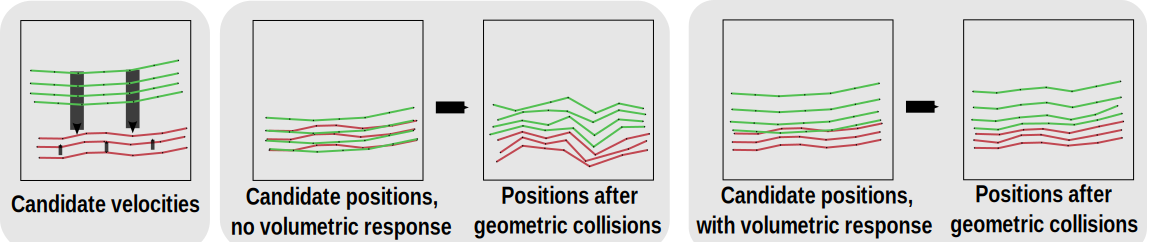
\includegraphics[width=.99\linewidth]{hair/figures/stacking}
  \caption{\label{fig:stacking} Collisions under stacking. A
    comparison of geometric collisions with (right) and without (left)
    volumetric preconditioning.}

%(left) Velocities from elastic and body forces. (middle) Without a volumetric response, many geometric collision iterations produce visual artifacts. (right) Geometric collisions preconditioned with a volumetric response cleanly resolve all collisions.} 
\end{figure}


Once step 3 is done, we have a velocity field that roughly considers
self-collision and global collisions; however, it misses fine details because it
has been computed at the coarser resolution of the grid. If we had only a few
hundred guides, repulsions might be a good option for removing the remaining
collisions, but at the densities of our examples, they become impractical.  This
is because repulsions are proximity based, so as density increases, the fact that
thickness must decrease means that the repulsions look smaller compared to the
velocities. Thus we turn to swept self-collisions to handle our fine collisions.

Geometric collisions have been studied extensively for cloth simulation because
they are essential for preventing visual artifacts. The current state of the art
is based on \cite{bridson:2002:cloth} which uses a three stage process to ensure
no collisions are missed. First, contact is preconditioned using penalty-based
repulsions that are small enough to prevent visual artifacts. Second,
self-collisions are applied to stop as much interpenetration as
possible. In this step, collisions are detected by coplanarity tests
between nearby point/face and edge/edge pairs, and impulses are
applied to colliding pairs.  As new collisions may have been created
by these impulses, this step is iterated over until all collisions are
resolved. Third, rigid groups (impact zones) are used as a final safety net,
postconditioning the collisions. Subsequent papers have typically focused on
improving the latter two components. For example \cite{sifakis:2008:cloth}
replaces the second step with a globally coupled collision scheme and
\cite{harmon:2008:cloth} improves rigid impact zones.

For cloth, improving collisions through better post-conditioning is a useful
technique because failures in repulsions and self-collisions typically do not
result in significant visual artifacts.  In hair, however, a deluge of
repulsions and collisions applied using relatively unstable edge/edge
interactions results in configurations that would be difficult to correct with a
better rigid group technique.  \cite{selle:2008:hair} mentions many of these
difficulties and in fact they resorted to turning off collisions in contact
cases to prevent these pitfalls.

In our implementation, we follow the collision algorithm in
\cite{bridson:2002:cloth} for edge/edge pairs. However, the placement
of our volume handling before applying self-collisions not only makes
finding a final collision free configuration possible, but
it actually preconditions the collision step--effectively replacing the repulsion step of
Bridson.  This allows us to prevent poor configurations before they create
visual artifacts in the self-collision and rigid group steps which is essential
in hair where the lack of stabilizing point/face interactions make collisions
potentially more damaging.  In fact, in many ways it is a better preconditioner
than proximity-based repulsions, because our volume formulation considers
velocities as well as positions. We illustrate the effectiveness of a
volumetric response to stacking collisions in Figure~\ref{fig:stacking}. 

\vspace{-2pt}
\section{Results}
\vspace{-4pt}

\begin{figure*}[htb]
\textsf{
%  \centering
%%  \includegraphics[width=.99\linewidth]{hair/images/tubes/tubes_1_row}\\
\begin{tabular}[t]{p{.20\linewidth}|p{.22\linewidth}p{.22\linewidth}p{.22\linewidth}}
 & \hspace{5pt}\textbf{Our Hybrid Method}& \hspace{5pt}\textbf{Lagrangian Collisions}& \hspace{5pt}\textbf{Eulerian
    Collisions} \\
%{\huge\textbf{Method \hbox{Comparison} and Timing}} 
\begin{minipage}{\linewidth}
Both Lagrangian collisions
  and our method successfully stop the falling bundle while the Eulerian collisions
  do not.
\end{minipage}
 & 
     \multicolumn{3}{l}{
\begin{minipage}{\linewidth}
\vspace{3pt}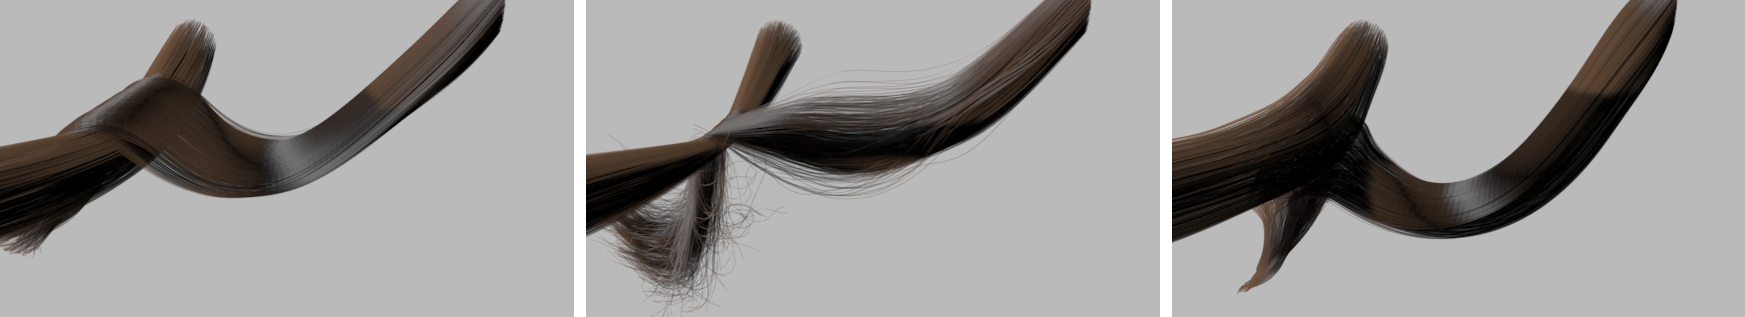
\includegraphics[width=.75\linewidth]{hair/images/tubes/tubes_2_row}
\vspace{3pt}   \end{minipage}}\\
\begin{minipage}{\linewidth}
Our method exhibits a more natural coupling which
  still exhibits high fidelity detail.
\end{minipage}
 &\multicolumn{3}{l}{\vspace{3pt}\begin{minipage}{\linewidth}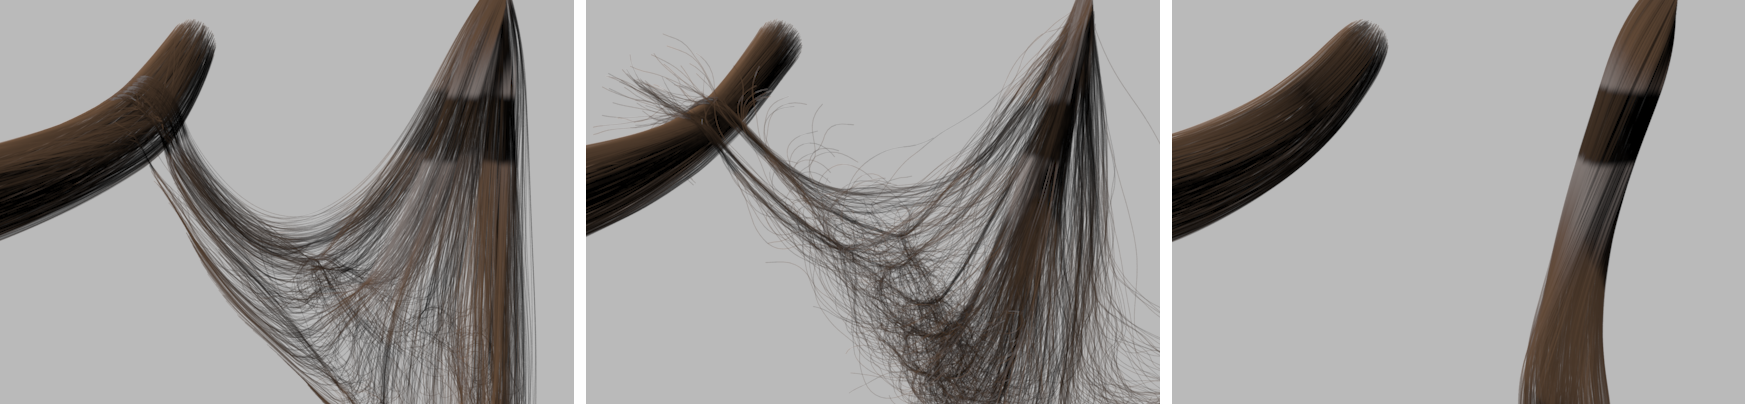
\includegraphics[width=.75\linewidth]{hair/images/tubes/tubes_3_row}\vspace{3pt}\end{minipage}}\\
%\hline
\hfill\textbf{Geometric collisions time} &\hspace{5pt}1.14 min/frame &\hspace{5pt}9.34 min/frame &\hspace{5pt}N/A \\
\hfill\textbf{Volume substep time} &\hspace{5pt}3.65 min/frame &\hspace{5pt}N/A & \hspace{5pt}3.55 min/frame \\
\hfill\textbf{Total time} & \hspace{5pt}7.97 min/frame &\hspace{5pt}13.63 min/frame &\hspace{5pt}5.67 min/frame \\
\end{tabular}
}
%
%%\begin{tabularOur Method&Lagrangian Collisions&Eulerian Collisions\end{tabular}
%%\hspace{70pt}\textbf{Our Method} \hfill \textbf{Lagrangian Collisions} \hfill \textbf{Eulerian Collisions}\hspace{70pt}
%%  \includegraphics[width=.99\linewidth]{hair/images/tubes/tubes_4_row}
  \caption{\label{fig:tubes} A cylindrical bundle of hairs is dropped on another
  bundle of suspended hairs with a timing table (2400 hairs). }
\end{figure*}

We have demonstrated our technique with a range of examples in our prototype
system; one can easily implement it with a standard Lagrangian hair simulator
and Eulerian fluid solver.  Examples are rendered with Renderman and standard hair
shading models. It would be feasible to apply the recent subsurface scattering and
shadowing acceleration techniques of
\cite{moon:2008:hair-render,zinke:2008:hair-render,bertails:2005:render}, some of
which might benefit from our rasterized volume.  While we
do not generate any additional strands at render time, traditional
interpolation or clumping techniques can naturally be utilized if more strands
are desired for rendering detail. A typical example uses a grid with
$60^3$ cells in the volumetric step; however, this number is
dynamically updated as the volume of hair changes shape.

We also demonstrate complex contact and collision
using a braid pattern consisting of 1500 hairs with approximately 100 particles
each in Figure~9.
The three hair sections begin in a very loose configuration with the top particle of
each hair fixed.  As gravity pulls the hairs downward, a braid pattern emerges
due to our Eulerian/Lagrangian collisions.
Figure~\ref{fig:char} shows our technique applied to an animated
character walking with 10,000 simulated hairs. 
Our last example (Figure~\ref{fig:tubes}) compares our method to
Lagrangian and Eulerian collisions alone. A bundle of 1200 hairs is draped
across a perpendicularly hanging bundle of 1200 more hairs (240,000
particles). Whereas purely Lagrangian collisions create highly active collision
impulses due to inadequate hair coupling, purely Eulerian collisions are overly damped and
fail to resolve the collisions.  Our result shows a moderate amount of coupling
from the volume together with fine details obtained with Lagrangian collisions.
Figure~\ref{fig:hold} shows that our method  compares favorably to real hair behavior.  

A comparison of runtimes for the three techniques shows the purely Eulerian
technique has the lowest average runtime per frame (5.6m).  Although our
method computes both volumetric and Lagrangian collisions, it is still
significantly faster (8m) per frame than
Lagrangian collisions alone (13.6m), showing the effectiveness of the Eulerian
divergence-free solve as a collision preconditioner.  A further breakdown of
timing can be found in Figure~\ref{fig:tubes}, and we note that the remainder
of time is spent on time integration.


We note that simulation time was about 15 minutes (26.9\% Lagrangian
collisions, 33.9\% volumetric, 39.2\% mass/ spring time integration)
per frame for the character in Figure~\ref{fig:char} on a single machine which is an
improvement over the 16-way parallel runtimes of \cite{selle:2008:hair}. 
The time step was determined by the mass spring Courant condition, though we found
in many examples that the volumetric step provided some extra stability,
allowing us to relax the time step restriction.

%tests, the average time step was between $7 \times 10^{-4}$ and $1.5
%\times%10^{-3}$ 

%\begin{table}[b!]
%  \centering 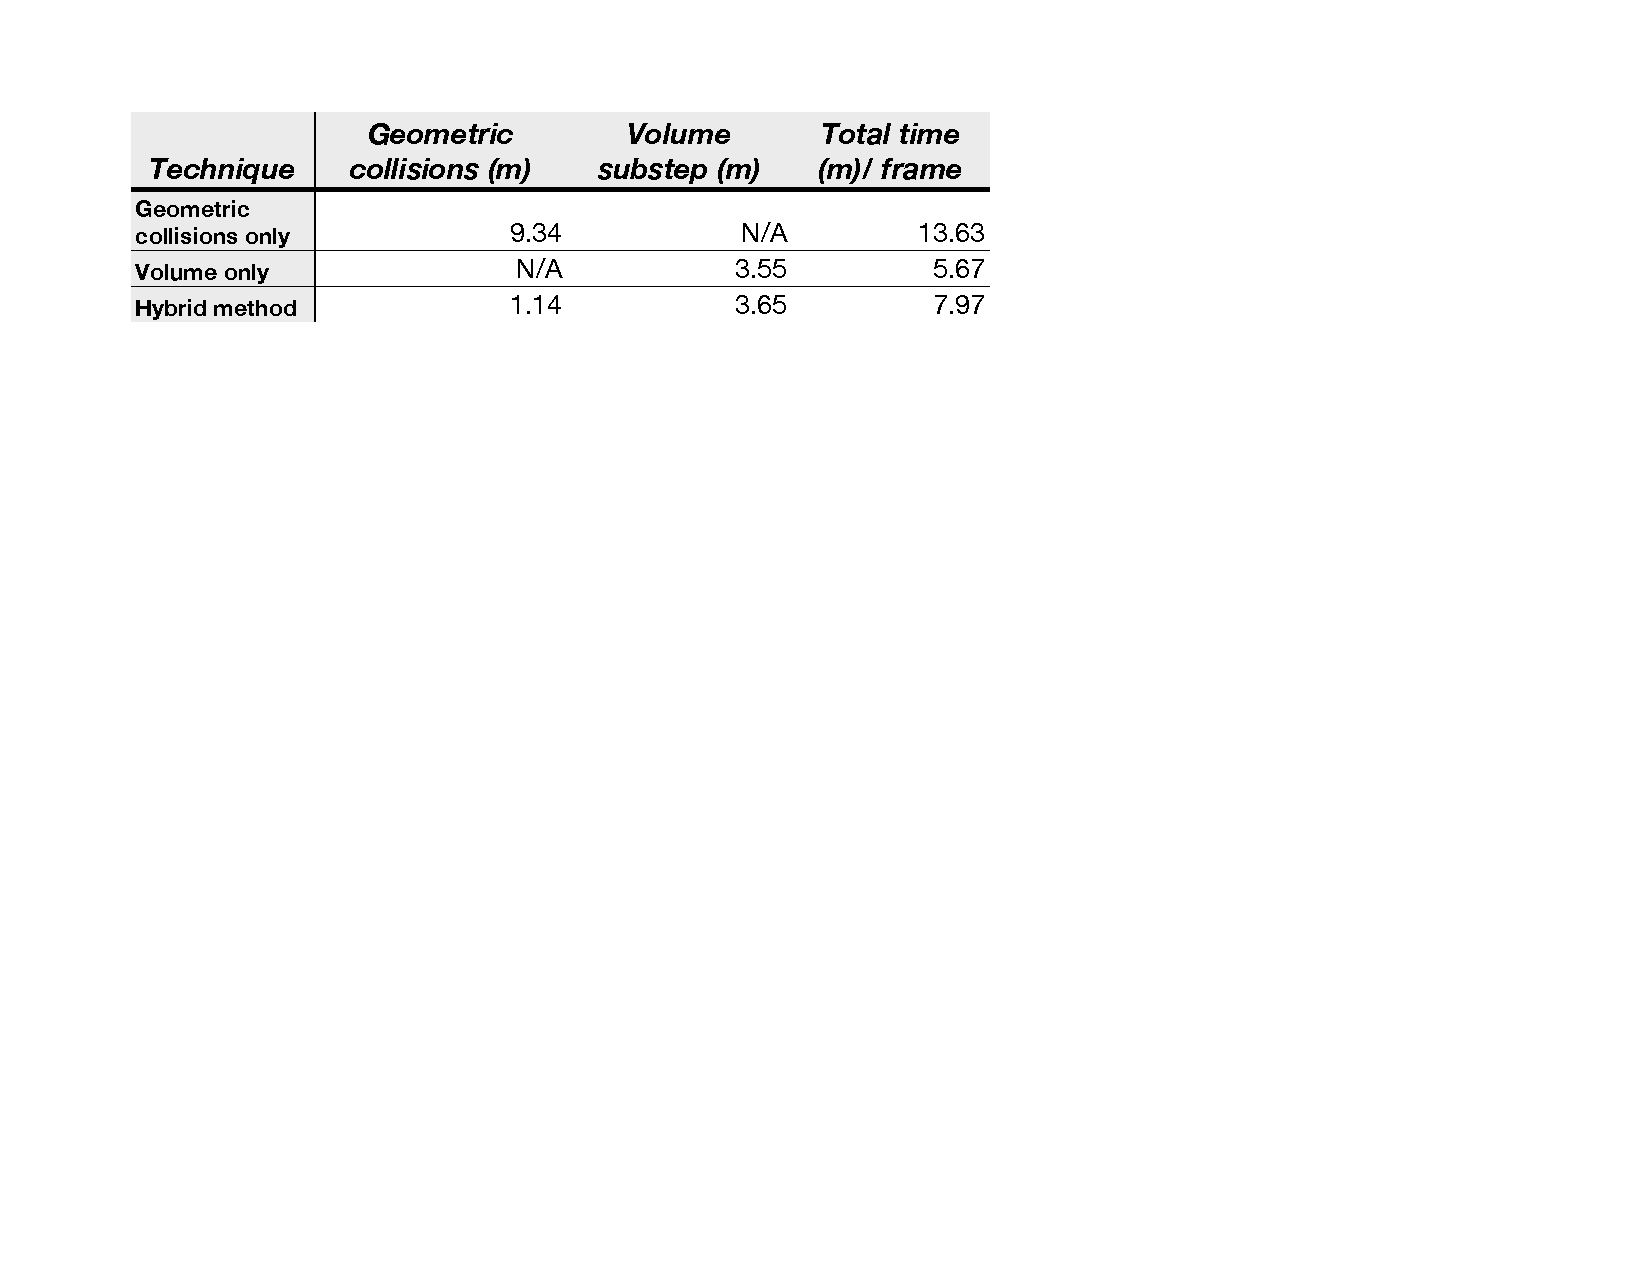
\includegraphics[width=.9\linewidth]{hair/figures/tube_times}
%  \caption{\label{table:tubes} A comparison of runtimes for purely Lagrangian,
%    purely Eulerian, and our hybrid technique on 2400 hairs. (See Fig~\ref{fig:tubes})} 
%\vspace{-5pt}
%\end{table}

\section{Discussion}
\vspace{-4pt}

\newcommand{\figurewidth}{1.8in}
\cutout{r} \shapepar[\figurewidth]{{0}
{0}b{-.8}\\
{.5}t{-1}{1}\\
{1}t{-1}{1}\\
{1.7}e{-.5}}
\begin{picture}(0,0)
\put
(-20,-210){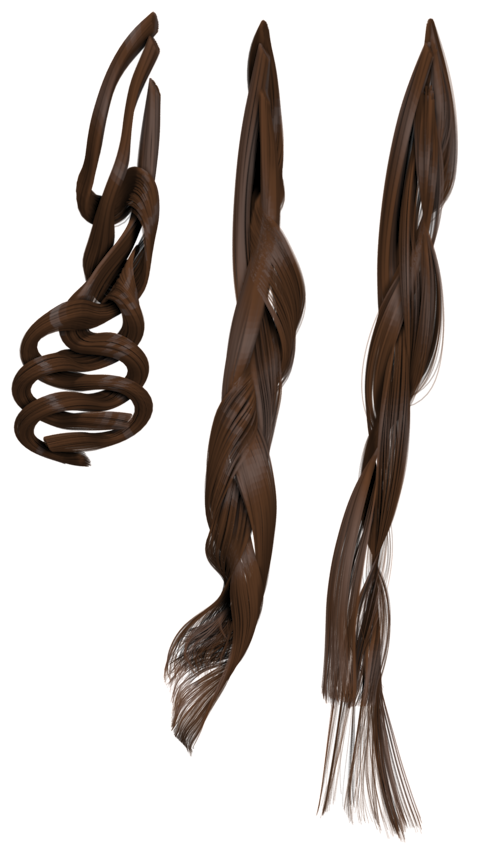
\includegraphics[width=\figurewidth]{hair/images/braidfigurenew}}
 \put(50,-220){\textbf{Figure
  9}}
\end{picture}

While we believe our technique makes high-fidelity interactions tractable, there
are some limitations.  We have not tried this method on non-straight hair as
straight hair tends to exhibit the most complicated stacking
configurations. Bridson's collision handling algorithm in
generalized coordinates may be difficult to apply because
impulses are given in maximal coordinates, and the associated generalized
coordinate response can be ambiguous. The FLIP impulse will be similarly
difficult to apply. Thus, in future work we plan to experiment with the maximal
coordinate mass-spring torsion model of \cite{selle:2008:hair}.
We note, however, that the braid simulation (1500 hairs, 150 particles
each) in Figure~9
shows both large and small scale interactions, showing promise for applications
of our method.  

In addition, the resolution of the
volume creates some numerical viscosity and in particular angular velocity
dissipation. This can be controlled by reducing the use of the volume (at the
expense of less efficiency) or by increasing the resolution of the
grid. Additionally, if the grid is too coarse, pieces of hair that become
severely tangled may not be able to separate. Similarly since friction is
modeled partially by viscosity (numerical and modeled), it is somewhat
inaccurate. So in the future we would like to investigate using an octree grid,
to allow different resolutions in different parts. For example, using the work of
\cite{ward:2003:modeling-hair-lod} in a large volume of hair, hair that is not
visible may not require a highly detailed velocity field.  Creating a level set
by applying a fast marching method to the previous timestep's density volume
could derive a refinement criterion. Parallelization of the grid rasterization,
Poisson solve, and FLIP application would also allow higher resolutions. We
expect these algorithms to map well to multicore architectures and graphics hardware. 
We are also interested in applying this technique to cloth as a
replacement to the Bridson repulsions to better precondition the cloth
collisions.


\vspace{-2pt}
\section{Conclusion}
\vspace{-4pt}

We have presented a technique that hybridizes Lagrangian and Eulerian hair
simulation techniques. Inspired by recent FLIP and SPH fluid technology, we show
that our model can be useful as a way of controlling the integration of volume
based forces. In addition we show how the volume can ease collision difficulties
with hair by acting as an improved preconditioner. We have shown that the
factorization of hair interaction into a coarse, globally-coupled phenomenon and a
highly detailed Lagrangian view is an effective strategy.  This improves
efficiency by allowing both types of behaviors to be captured in the most
natural way possible. 


